\documentclass[usenames,dvipsnames,aspectratio=169]{beamer}
\usepackage{../common/prg}

\title[4. előadás]{Programozás}
\subtitle{(GKxB\_INTM114)}

\begin{document}

%1
\begin{frame}[plain]
  \titlepage
  \logoalul
\end{frame}

%2
\section{Lebegőpontos típusok, egész- és lebegőpontos konstansok}
\subsection{Lebegőpontos konstansok (literálok)}
\begin{frame}
  \begin{columns}[c]
    \column{0.3\linewidth}
      \hfill 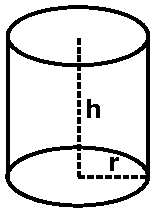
\includegraphics{henger.pdf}\\
    \column{0.7\linewidth}
      Feladat:
      \begin{enumerate}
        \item Beolvasandó a henger magassága és alapjának sugara
        \item Kiszámítandó a henger felszíne, térfogata\\
          $V = r^2\pi h$\\
          $S = 2r\pi h + 2r^2\pi = 2r\pi(r+h)$\\
      \end{enumerate}
      \vfill
  \end{columns}
  \begin{center}
    \begin{tabular}{llll}
      Típus & Méret & Számábrázolási határok & Pontosság\\ \hline \noalign{\smallskip}
      float & 4 bájt & $\pm3,4\cdot10^{-38}$ -- $\pm3,4\cdot10^{+38}$ & 6-7 dec. jegy\\
      double & 8 bájt & $\pm1,7\cdot10^{-308}$ -- $\pm1,7\cdot10^{+308}$ & 15-16 dec. jegy\\
      long double & 10 bájt & $\pm1,2\cdot10^{-4932}$ -- $\pm1,2\cdot10^{+4932}$ & 19 dec. jegy
    \end{tabular}
  \end{center}
\end{frame}

%3
\begin{frame}
  \begin{exampleblock}{\textattachfile{henger.cpp}{henger.cpp}}
  \footnotesize
  \lstinputlisting[style=cpp,numbers=left]{henger.cpp}
\end{exampleblock}
\end{frame}

%4
\begin{frame}
  \kiemel{Lebegőpontos} konstansok főbb tulajdonságai
  \begin{itemize}
    \item ábrázolási határok $\to$ \texttt{cfloat} (\texttt{float.h}), pl. 
    \begin{description}[\texttt{DBL\_MIN}]
      \item[\texttt{DBL\_MIN}] a \texttt{double} típussal ábrázolható legkisebb pozitív szám
      \item[\texttt{DBL\_MAX}] a \texttt{double} típussal ábrázolható legnagyobb véges szám
    \end{description}
    \item mantisszából elhagyható az egész- vagy a törtrész, de \kiemel{mindkettő nem}!
    \item elhagyható a tizedes pont vagy az exponens (\texttt{e, E}) rész, de \kiemel{mindkettő nem}!
    \item utótag nélkül a belső ábrázolás \texttt{double}
  \end{itemize}
\end{frame}

%5
\begin{frame}
  \begin{itemize}
    \item Utótagok a konstans belső ábrázolásának megváltoztatásához:
    \begin{itemize}
      \item \texttt{f}, \texttt{F} (\texttt{float})
      \item \texttt{l}, \texttt{L} (\texttt{long double})
    \end{itemize}
  \end{itemize}
  \begin{exampleblock}{Néhány lebegőpontos konstans}
    -5., .3, 5.3, -5e4, 5.67E-12, -1.23e-4l, 5.F
  \end{exampleblock}
   A \texttt{cmath} (\texttt{math.h}) néhány (\hiv{\href{https://en.cppreference.com/w/cpp/header/numbers}{nem feltétlenül szabványosított}}) konstansa
  \begin{itemize}
    \item \texttt{M\_E} -- Euler-konstans
    \item \texttt{M\_PI} -- $\pi$ értéke
    \item \texttt{M\_SQRT2} -- $\sqrt{2}$
  \end{itemize}
\end{frame}

%6
\subsection{Egész konstansok (literálok)}
\begin{frame}[fragile]
  Az \kiemel{egész} konstansok főbb tulajdonságai
  \begin{itemize}
    \item megadható decimális, oktális (\texttt{0}\dots) és hexadecimális (\texttt{0x}\dots, \texttt{0X}\dots) alakban
    \item \hiv{\href{https://en.cppreference.com/w/cpp/language/integer\_literal}{utótagok}} a konstans típusának megváltoztatásához:
    \begin{itemize}
      \item \texttt{u}, \texttt{U} (unsigned)
      \item \texttt{l}, \texttt{L} (long)
      \item \texttt{ll}, \texttt{LL} (long long)
      \item \texttt{z}, \texttt{Z} (std::size\_t)
    \end{itemize}
  \end{itemize}
  \begin{exampleblock}{Egész típusú változók és konstansok}
    \begin{verbatim}
int i = 1;                unsigned ui = 8u;
int j = 010;  /* == 8 */  long li = 16L;
int k = 0x2A; /* == 42 */ unsigned long uli = 666Ul;
\end{verbatim}
  \end{exampleblock}
\end{frame}

%7
\begin{frame}
  \begin{itemize}
    \item platformfüggő méretű egész típusok ábrázolási korlátai $\to$ \texttt{climits} (\texttt{limits.h})
    \item rögzített szélességű egész típusok $\to$ \texttt{cstdint} (\texttt{stdint.h}).
  \end{itemize}
  \begin{block}{\texttt{climits} részletek}
    \#define SCHAR\_MIN     (-128)\\
    \#define UCHAR\_MAX     255\\
    \#define SHRT\_MAX      32767\\
    \#define INT\_MAX       2147483647\\
    \#define ULONG\_MAX     18446744073709551615UL
  \end{block}
\end{frame}

%8
\subsection{Matematikai függvények}
\begin{frame}
  \begin{exampleblock}{\textattachfile{masodfoku.cpp}{masodfoku.cpp} Másodfokú egyenlet megoldóképlete: $x_{1,2} = \frac{-b\pm\sqrt{b^2 - 4ac}}{2a}$}
    \tiny
    \vspace{-.2cm}
    \lstinputlisting[style=cpp,numbers=left]{masodfoku.cpp}
    \vspace{-.2cm}
  \end{exampleblock}
\end{frame}

%9
\begin{frame}
  \begin{itemize}
    \item Szabványos függvénykönyvtárak $\to$ hordozhatóság
    \item Beszerkesztendő fejfájl: \texttt{cmath} (\texttt{math.h})
    \item Függvények paramétereinek típusa és visszatérési értéke többnyire \texttt{double}
    \item Trigonometrikus fv.-ek paramétere és visszatérési értéke \kiemel{radiánban} értendő
  \end{itemize}
\end{frame}

%10
\begin{frame}
  Néhány gyakran használt \hiv{\href{https://en.cppreference.com/w/cpp/numeric/math}{matematikai függvény}}
  \vfill
  \footnotesize
  \begin{tabular}{p{.4\textwidth}p{.5\textwidth}}
    Prototípus & Funkció\\ \hline
    \texttt{double ceil(double x)} & Az x-nél nagyobb egészek közül a legkisebbet adja\\
    \texttt{double cos(double x)} & koszinusz\\
    \texttt{double cosh(double x)} & hiperbolikus koszinusz\\
    \texttt{double exp(double x)} & exponenciális fv.\\
    \texttt{double fabs(double x)} & abszolút érték\\
    \texttt{double fmod(double x, double~y)} & osztás lebegőpontos maradékát adja\\
    \texttt{double log(double x)} & természetes alapú logaritmus\\
    \texttt{double log10(double x)} & 10-es alapú logaritmus\\
    \texttt{double pow(double x, double~y)} & hatványozás\\
    \texttt{double sqrt(double x)} & négyzetgyökvonás
  \end{tabular}
\end{frame}

%11
\begin{frame}
  \begin{exampleblock}{\textattachfile{haromszog4.cpp}{haromszog4.cpp}}
    \tiny
    \lstinputlisting[style=cpp,numbers=left]{haromszog4.cpp}
  \end{exampleblock}
\end{frame}

%12
\section{Típuskonverziók}
\subsection{Implicit típuskonverziók}
\begin{frame}
  \begin{exampleblock}{\textattachfile{haromszog5.cpp}{haromszog5.cpp}}
    \small
    \lstinputlisting[style=cpp,linerange={9-16},numbers=left,firstnumber=9]{haromszog5.cpp}
  \end{exampleblock}
  \begin{block}{Kimenet}
Adja meg egy haromszog oldalhosszait!\\
\kiemel{65} oldal hossza:
  \end{block}
\end{frame}

%13
\begin{frame}
  \kiemel{Implicit} típuskonverzió: kétoperandusos műveleteknél, ha az operandusok típusa eltér. Általában a ,,pontosabb''
típusra alakít. Szabályok:
  \begin{center}
    \[
      \left\downarrow\mbox{
      \begin{tabular}{ll}
        egyik operandus & másik operandus\\ \hline
        \texttt{long double} & \emph{bármi}$\to$\texttt{long double}\\
        \texttt{double} & \emph{bármi}$\to$\texttt{double}\\
        \texttt{float} & \emph{bármi}$\to$\texttt{float}\\
        \emph{egész-előléptetés} & \emph{egész-előléptetés}\\
        \texttt{unsigned long} & \emph{bármi}$\to$\texttt{unsigned long}\\
        \texttt{long}$\to$(\texttt{unsigned}) \texttt{long} & \texttt{unsigned int}$\to$(\texttt{unsigned})
        \texttt{long}\\
        \texttt{long} & \emph{bármi}$\to$\texttt{long}\\
        \texttt{unsigned int} & \emph{bármi}$\to$\texttt{unsigned int}\\
        int & int
      \end{tabular}}
      \right.
    \]
  \end{center}
\end{frame}

%14
\begin{frame}
  \kiemel{Egész-előléptetés} (integral promotion)
  \begin{center}
    \footnotesize
    \begin{tabular}{llp{.56\textwidth}}
      Régi típus & Új típus & Átalakítási módszer\\ \hline
      \texttt{char} & \texttt{int} & Alapértelmezett (signed/unsigned) char típustól függően.\\
      \texttt{unsigned char} & \texttt{int} & Felső bájtok feltöltése zérus bitekkel.\\
      \texttt{signed char} & \texttt{int} & Előjel kiterjesztése a felső bájtokra.\\
      \texttt{short int} & \texttt{int} & Előjel kiterjesztés.\\
      \texttt{unsigned short} & \texttt{unsigned int} & Feltöltés zérus bitekkel.\\
    \end{tabular}
  \end{center}
  \vfill
  Figyelem!
  \begin{itemize}
    \item A konverzió időigényes!
    \item Karakterlánc sosem alakul aritmetikai értékké!
  \end{itemize}
\end{frame}

%15
\subsection{Explicit típuskonverzió (Type cast)}
\begin{frame}
  \begin{exampleblock}{\textattachfile{haromszog6.cpp}{haromszog6.cpp}}
    \scriptsize
    \lstinputlisting[style=cpp,linerange={9-17},numbers=left,firstnumber=9]{haromszog6.cpp}
  \end{exampleblock}
  \begin{block}{Kimenet}
Adja meg egy haromszog oldalhosszait!\\
\kiemel{A} oldal hossza:
  \end{block}
\end{frame}

%16
\begin{frame}
  \begin{columns}[c]
    \column{0.62\linewidth}
      \begin{exampleblock}{\textattachfile{fahrCels1.cpp}{fahrCels1.cpp}}
        \meret{9}
        \lstinputlisting[style=cpp,numbers=left]{fahrCels1.cpp}
      \end{exampleblock}
    \column{0.33\linewidth}
      Fahrenheit -- Celsius átváltás\\ $C = \frac{5}{9}(F-32)$
      \begin{block}{Kimenet}
        \scriptsize
        Fahrenheit --> Celsius\\
        Fahrenheit: 72\\
        Celsius: 0\\
      \end{block}
  \end{columns}
\end{frame}

%17
\begin{frame}
  \begin{columns}[T]
    \column{0.45\linewidth}
      \begin{exampleblock}{\textattachfile{fahrCels2.cpp}{fahrCels2.cpp}}
        \scriptsize
        \vspace{-.2cm}
        \lstinputlisting[style=cpp,numbers=left,firstline=10,lastline=11,firstnumber=10]{fahrCels2.cpp}
        \vspace{-.2cm}
      \end{exampleblock}
      \begin{block}{Kimenet}
        \scriptsize
        Celsius: 22.2222\\
      \end{block}
      \begin{exampleblock}{\textattachfile{fahrCels4.cpp}{fahrCels4.cpp}}
        \scriptsize
        \vspace{-.2cm}
        \lstinputlisting[style=cpp,numbers=left,firstline=10,lastline=11,firstnumber=10]{fahrCels4.cpp}
        \vspace{-.2cm}
      \end{exampleblock}
      \begin{block}{Kimenet}
        \scriptsize
        Celsius: 22.2222\\
      \end{block}
    \column{0.45\linewidth}
      \begin{exampleblock}{\textattachfile{fahrCels3.cpp}{fahrCels3.cpp}}
        \scriptsize
        \vspace{-.2cm}
        \lstinputlisting[style=cpp,numbers=right,firstline=10,lastline=11,firstnumber=10]{fahrCels3.cpp}
        \vspace{-.2cm}
      \end{exampleblock}
      \begin{block}{Kimenet}
        \scriptsize
        Celsius: 22.2222\\
      \end{block}
      \begin{exampleblock}{\textattachfile{fahrCels5.cpp}{fahrCels5.cpp}}
        \scriptsize
        \vspace{-.2cm}
        \lstinputlisting[style=cpp,numbers=right,firstline=10,lastline=11,firstnumber=10]{fahrCels5.cpp}
        \vspace{-.2cm}
      \end{exampleblock}
      \begin{block}{Kimenet}
        \scriptsize
        Celsius: 0\\
      \end{block}
  \end{columns}
\end{frame}


%18
\section{Vezérlési szerkezetek}
\subsection{A feltételes operátor}
\begin{frame}
  Feltételes operátor: \kiemel{\texttt{?:}}
  \begin{exampleblock}{Szelekciós tevékenység}
    if(\kiemel{logikaiKifejezes}) \{\\
    \hspace{0.5cm} valtozo = \kiemelZ{ertekHaIgaz};\\
    \} else \{\\
    \hspace{0.5cm} valtozo = \kiemelN{ertekHaHamis};\\
    \}
  \end{exampleblock}
  \begin{exampleblock}{Feltételes operátor}
    valtozo = \kiemel{logikaiKifejezes} ? \kiemelZ{ertekHaIgaz} : \kiemelN{ertekHaHamis};
  \end{exampleblock}
\end{frame}

%19
\begin{frame}
  \begin{exampleblock}{\textattachfile{haromszog7.cpp}{haromszog7.cpp}}
    \tiny
    \lstinputlisting[style=cpp,linerange={18-19},numbers=left,firstnumber=18]{haromszog7.cpp}
  \end{exampleblock}
  \begin{columns}[T]
    \column{0.46\linewidth}
      \begin{exampleblock}{\textattachfile{abszolut1.cpp}{abszolut1.cpp}}
        \tiny
        \vspace{-.2cm}
        \lstinputlisting[style=cpp,numbers=left]{abszolut1.cpp}
        \vspace{-.2cm}
      \end{exampleblock}
    \column{0.46\linewidth}
      \begin{exampleblock}{\textattachfile{abszolut2.cpp}{abszolut2.cpp}}
        \tiny
        \vspace{-.2cm}
        \lstinputlisting[style=cpp,numbers=right]{abszolut2.cpp}
        \vspace{-.2cm}
      \end{exampleblock}
  \end{columns}
\end{frame}

%20
\subsection{Új operátorok helye a precedencia táblázatban}
\begin{frame}
  \begin{columns}[c]
    \column{.45\textwidth}
    Operátorok precedenciája és asszociativitása
    \column{.5\textwidth}
      \meret{9}
      \begin{tabular}{ll}
      Operátor & Asszociativitás \\ \hline\hline
      a++ a$--$ & \multirow{2}{*}{balról jobbra} \\ 
      \kiemel{type() fn() array[]} & \\ \hline
      ++a $--$a & \multirow{5}{*}{jobbról balra} \\
      +a $-$a & \\
      ! & \\
      \kiemel{(type)} & \\
      sizeof & \\ \hline
      a*b a/b a\%b & \multirow{6}{*}{balról jobbra} \\
      a+b a$-$b & \\
      < <= > >= & \\
      == != & \\
      \&\& & \\
      || & \\ \hline
      \kiemel{a?b:c} & \multirow{2}{*}{jobbról balra}\\
      = += $-$= *= /= \%= & \\ \hline
      , & balról jobbra \\ \hline
      \end{tabular}
  \end{columns}
\end{frame}

%21
\subsection{\texttt{for} (növekményes) ciklus}
\begin{frame}
  \scriptsize
  \texttt{for(}<\emph{init-kifejezés}>\texttt{;} <\emph{kifejezés}>\texttt{;} <\emph{léptető-kifejezés}>\texttt{)} 
\emph{utasítás}
  \begin{enumerate}
    \item \emph{init-kifejezés} végrehajtása, ha megadták
    \item \emph{utasítás} végrehajtása, ha \emph{kifejezés} igaz; lehet összetett
    \item \emph{léptető-kifejezés} végrehajtása, ha megadták, majd ugrás a 2. pontra
  \end{enumerate}
  \vfill
  Tipikus forgatókönyv:
  \begin{exampleblock}{while}
    \kiemel{ciklusValtozo = kezdoErtek;}\\
    while(\kiemelZ{ciklusValtozo < vegErtek}) \{\\
      \hspace{0.5cm} ciklusMag;\\
      \hspace{0.5cm} \kiemelN{ciklusValtozo += lepes;}\\
    \}\\
  \end{exampleblock}
  \begin{exampleblock}{for}
    for(\kiemel{ciklusValtozo=kezdoErtek}; \kiemelZ{ciklusValtozo<vegErtek}; \kiemelN{ciklusValtozo += lepes}) \{\\
      \hspace{0.5cm} ciklusMag;\\
    \}\\
  \end{exampleblock}
\end{frame}

%22
\begin{frame}
  \emph{N} darab szám beolvasása, tárolása, kiírása fordított sorrendben
  \begin{columns}[T]
    \column{0.45\linewidth}
      \begin{exampleblock}{\textattachfile{forditva1.cpp}{forditva1.cpp}}
        \scriptsize
        \lstinputlisting[style=cpp,numbers=left,linerange={7-15},firstnumber=7]{forditva1.cpp}
      \end{exampleblock}
    \column{0.45\linewidth}
      \begin{exampleblock}{\textattachfile{forditva3.cpp}{forditva3.cpp}}
        \scriptsize
        \lstinputlisting[style=cpp,numbers=right,linerange={7-15},firstnumber=7]{forditva3.cpp}
      \end{exampleblock}
  \end{columns}
\end{frame}

%23
\begin{frame}
  Tízes számrendszerbeli szám átalakítása kettes számrendszerbelivé
  \begin{columns}[T]
    \column{0.45\linewidth}
      \begin{exampleblock}{\textattachfile{kettes2.cpp}{kettes2.cpp}}
        \meret{6}
        \lstinputlisting[style=cpp,numbers=left]{kettes2.cpp}
      \end{exampleblock}
    \column{0.45\linewidth}
      \begin{exampleblock}{\textattachfile{kettes3.cpp}{kettes3.cpp}}
        \meret{6}
        \lstinputlisting[style=cpp,numbers=right]{kettes3.cpp}
      \end{exampleblock}
  \end{columns}
\end{frame}

%24
\begin{frame}
  Szó megfordítása helyben
  \begin{columns}[T]
  \column{0.45\linewidth}
    \begin{exampleblock}{\textattachfile{szofordit1.cpp}{szofordit1.cpp}}
      \tiny
      \vspace{-.2cm}
      \lstinputlisting[style=cpp,numbers=left]{szofordit1.cpp}
      \vspace{-.2cm}
    \end{exampleblock}
  \column{0.45\linewidth}
    \begin{exampleblock}{\textattachfile{szofordit2.cpp}{szofordit2.cpp}}
      \tiny
      \vspace{-.2cm}
      \lstinputlisting[style=cpp,numbers=right]{szofordit2.cpp}
      \vspace{-.2cm}
    \end{exampleblock}
  \end{columns}
\end{frame}

\end{document}